\section{Z branching ratios.}

Starting from the matrix element, work through the calculation of the $Z \to f \bar{f}$ partial decay rate, expressing the answer in terms of the vector and axial-vector couplings of $Z$. Taking $\sin^2(\theta_W) = 0.2315$, show that

\begin{align*}
    R_\mu &= \frac{\Gamma(Z \to \mu^+ \mu^-)}{\Gamma(Z \to \text{hadrons})} \approx \frac{1}{20}
\end{align*}

\begin{align*}
    \hline
\end{align*}

Let's begin with a Feynman diagram:
\begin{center}
    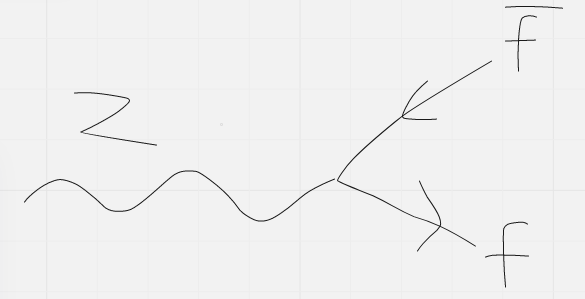
\includegraphics[width=0.3\textwidth]{q5_1.png}
\end{center}

And now construct a matrix element with all the terms:
\begin{itemize}
    \item Incoming $Z$: $\epsilon_\mu(p_Z)$
    \item $Z \to f\bar{f}$ vertex: $-i\frac{1}{2}g_Z \gamma^\mu [c_V - c_A \gamma^5]$
    \item Outgoing $f$: $\bar{u}(p_f)$
    \item Outgoing $\bar{f}$: $v(p_{\bar{f}})$
\end{itemize}

\begin{align*}
    -i\mathcal{M} &= \epsilon_\mu(p_Z)\bar{u}(p_f)\left(-i\frac{1}{2}g_Z \gamma^\mu [c_V - c_A \gamma^5]\right)v(p_{\bar{f}}) \\
    &= \epsilon_\mu(p_Z)\bar{u}(p_f)\left(-i\frac{1}{2}g_Z \gamma^\mu [c_V - c_A \gamma^5]\right)v(p_{\bar{f}}) \\
    \mathcal{M} &= \epsilon_\mu(p_Z)\bar{u}(p_f)\frac{1}{2}g_Z \gamma^\mu [c_V - c_A \gamma^5]v(p_{\bar{f}}) \\
\end{align*}

This is a chiral interaction, take the relativistic limit where chirality $\approx$ helicity, and see which currents are zero:

\begin{align*}
    \bar{u}_R \gamma^\mu [c_V - c_A \gamma^5]v_R &= \overline{P_R u} \gamma^\mu [c_V - c_A \gamma^5]v_R \\
    &= u^\dagger P_R \gamma^0 \gamma^\mu [c_V - c_A \gamma^5]v_R \\
    &= u^\dagger \frac{1}{2}(1 + \gamma^5) \gamma^0 \gamma^\mu [c_V - c_A \gamma^5] v_R \\
    &= u^\dagger \gamma^0 \gamma^\mu [c_V - c_A \gamma^5]\frac{1}{2}(1 + \gamma^5) v_R \\
    &= u^\dagger \gamma^0 \gamma^\mu [c_V - c_A \gamma^5]P_R v_R \\
    &= u^\dagger \gamma^0 \gamma^\mu [c_V - c_A \gamma^5](0) \\
    &= 0
\end{align*}
(we used the commutation property $[\gamma^5, \gamma^\mu] = 0$ here)

\begin{align*}
    \bar{u}_L \gamma^\mu [c_V - c_A \gamma^5]v_L &= \overline{P_L u} \gamma^\mu [c_V - c_A \gamma^5]v_L \\
    &= u^\dagger P_L \gamma^0 \gamma^\mu [c_V - c_A \gamma^5]v_L \\
    &= u^\dagger \frac{1}{2}(1 - \gamma^5) \gamma^0 \gamma^\mu [c_V - c_A \gamma^5] v_L \\
    &= u^\dagger \gamma^0 \gamma^\mu [c_V - c_A \gamma^5]\frac{1}{2}(1 - \gamma^5) v_L \\
    &= u^\dagger \gamma^0 \gamma^\mu [c_V - c_A \gamma^5]P_L v_L \\
    &= u^\dagger \gamma^0 \gamma^\mu [c_V - c_A \gamma^5](0) \\
    &= 0
\end{align*}


\begin{align*}
    \bar{u}_R \gamma^\mu [c_V - c_A \gamma^5]v_L &= \overline{P_R u} \gamma^\mu [c_V - c_A \gamma^5]v_L \\
    &= u^\dagger P_R \gamma^0 \gamma^\mu [c_V - c_A \gamma^5]v_L \\
    &= u^\dagger \frac{1}{2}(1 + \gamma^5) \gamma^0 \gamma^\mu [c_V - c_A \gamma^5] v_L \\
    &= u^\dagger \gamma^0 \gamma^\mu [c_V - c_A \gamma^5]\frac{1}{2}(1 + \gamma^5) v_L \\
    &= u^\dagger \gamma^0 \gamma^\mu [c_V - c_A \gamma^5]P_R v_L \\
    &= u^\dagger \gamma^0 \gamma^\mu [c_V - c_A \gamma^5]v_L \\
    &\neq 0
\end{align*}

\begin{align*}
   \epsilon_\mu \bar{u}_R \gamma^\mu [c_V - c_A \gamma^5]v_L &= (E_f+m_f)\begin{pmatrix}
        c & s & -c & -s
    \end{pmatrix} \gamma^3 (c_V - c_A)\begin{pmatrix}
        c \\ -s \\ c \\ -s \\
    \end{pmatrix} \\
    &= (E_f+m_f)(c_V - c_A)\begin{pmatrix}
        c & s & -c & -s
    \end{pmatrix} \begin{pmatrix}
        0 & 0 & 1 & 0 \\
        0 & 0 & 0 & -1 \\
        -1 & 0 & 0 & 0 \\
        0 & 1 & 0 & 0 \\
    \end{pmatrix} \begin{pmatrix}
        c \\ -s \\ c \\ -s \\
    \end{pmatrix} \\
    &= (E_f+m_f)(c_V - c_A)\begin{pmatrix}
        c & s & -c & -s
    \end{pmatrix} \begin{pmatrix}
        c \\
        s \\
        -c \\
        -s \\
    \end{pmatrix} \\
    &= (E_f+m_f)(c_V - c_A)2(c^2 + s^2) \\
    &= 2(E_f+m_f)(c_V - c_A) \\
\end{align*}
(Used the polarization $\epsilon_\mu = (0,0,0,1)$)


\begin{align*}
    \bar{u}_L \gamma^\mu [c_V - c_A \gamma^5]v_R &= \overline{P_L u} \gamma^\mu [c_V - c_A \gamma^5]v_R \\
    &= u^\dagger P_L \gamma^0 \gamma^\mu [c_V - c_A \gamma^5]v_R \\
    &= u^\dagger \frac{1}{2}(1 - \gamma^5) \gamma^0 \gamma^\mu [c_V - c_A \gamma^5] v_R \\
    &= u^\dagger \gamma^0 \gamma^\mu [c_V - c_A \gamma^5]\frac{1}{2}(1 - \gamma^5) v_R \\
    &= u^\dagger \gamma^0 \gamma^\mu [c_V - c_A \gamma^5]P_L v_R \\
    &= u^\dagger \gamma^0 \gamma^\mu [c_V - c_A \gamma^5]v_R \\
    &\neq 0
\end{align*}


\begin{align*}
    \epsilon_\mu \bar{u}_L \gamma^\mu [c_V - c_A \gamma^5]v_R &= (E_f+m_f)\begin{pmatrix}
        -s & c & -s & c
    \end{pmatrix} \gamma^3 (c_V + c_A)\begin{pmatrix}
        -s \\ -c \\ s \\ c \\
    \end{pmatrix} \\
    &= (E_f+m_f)(c_V + c_A)\begin{pmatrix}
        -s & c & -s & c
    \end{pmatrix} \begin{pmatrix}
        0 & 0 & 1 & 0 \\
        0 & 0 & 0 & -1 \\
        -1 & 0 & 0 & 0 \\
        0 & 1 & 0 & 0 \\
    \end{pmatrix} \begin{pmatrix}
        -s \\ -c \\ s \\ c \\
    \end{pmatrix} \\
    &= (E_f+m_f)(c_V + c_A)\begin{pmatrix}
        -s & c & -s & c
    \end{pmatrix} \begin{pmatrix}
        s \\
        -c \\
        s \\
        -c \\
    \end{pmatrix} \\
    &= (E_f+m_f)(c_V + c_A)2(s^2+c^2) \\
    &= 2(E_f+m_f)(c_V + c_A) \\
\end{align*}

\begin{align*}
    |\mathcal{M}|^2 &= |\mathcal{M}_{LR}|^2 + |\mathcal{M}_{RL}|^2 \\
    &= 4g_Z^2(E_f+m_f)^2[(c_V + c_A)^2 + (c_V - c_A)^2] \\
    &= g_Z^2(2E_f)^2[(c_V + c_A)^2 + (c_V - c_A)^2] \\
    &= g_Z^2 E_Z^2[c_V^2 + c_A^2] \\
    &= g_Z^2 m_Z^2(c_V^2 + c_A^2) \\
\end{align*}

\begin{align*}
    \implies \expval{|\mathcal{M}|^2} &= \frac{1}{3}g_Z^2 m_Z^2(c_V^2 + c_A^2)
\end{align*}

Then using Fermi's golden rule and assuming the masses of the decay products are negligible compared to their energies (also noting $M$ has no spatial dependence),
\begin{align*}
    \Gamma &= \frac{p^*}{32\pi^2 m_Z^2} \int \expval{|M|^2} d\Omega^* \\
    &= \frac{p^*}{32\pi^2 m_Z^2} 4\pi \expval{|M|^2} \\
    &= \frac{p^*}{8\pi m_Z^2} \expval{|M|^2} \\
    &= \frac{p^*}{8\pi }\frac{1}{3} (c_V^2 + c_A^2) g_Z^2 \\
    &\approx \frac{m_Z/2}{8\pi }\frac{1}{3} (c_V^2 + c_A^2) g_Z^2 \\
    &= \frac{g_Z^2 m_Z}{48\pi} (c_V^2 + c_A^2) \\
\end{align*}

In the ratio later the constants will cancel, so consider only the $c_V^2 + c_A^2$ terms. Using table 15.1, for $\mu$ we have:
\begin{align*}
    c_V &= -0.04 \\
    c_A &= -\frac{1}{2} \\
    c_V^2 + c_A^2 &= 0.2516 \\
\end{align*}

For $u/c/t$:
\begin{align*}
    c_V &= +0.19 \\
    c_A &= +\frac{1}{2} \\
    c_V^2 + c_A^2 &= 0.2861 \\
\end{align*}

and $d/s/b$:
\begin{align*}
    c_V &= -0.35 \\
    c_A &= -\frac{1}{2} \\
    c_V^2 + c_A^2 &= 0.3725 \\
\end{align*}

Note that $Z$ cannot actually decay into tauons due to mass constraints, so in the following equation we exclude $t$. Also since there are three quark colours, we have factors of 3 below.

\begin{align*}
    R_\mu &= \frac{\Gamma(Z \to \mu^+ \mu^-)}{\Gamma(Z \to \text{hadrons})} \\
    &= \frac{\Gamma(Z \to \mu^+ \mu^-)}{\Gamma(Z \to \text{quarks except t})} \\
    &= \frac{\Gamma(Z \to \mu^+ \mu^-)}{3\Gamma(Z \to u\bar{u}) + 3\Gamma(Z \to c\bar{c}) + 3\Gamma(Z \to d\bar{d})+ 3\Gamma(Z \to s\bar{s})+ 3\Gamma(Z \to b\bar{b})} \\
    &= \frac{\Gamma(Z \to \mu^+ \mu^-)}{6\Gamma(Z \to u\bar{u}) + 9\Gamma(Z \to d\bar{d})} \\
    &= \frac{0.2516}{6(0.2861) + 9(0.3725)} \\
    &= 0.0496340573 \\
    &\approx 0.05 \\
    &= \frac{1}{20} \\
\end{align*}
